\documentclass[12pt]{article}
\usepackage[UTF8]{ctex} % using Chinese

\usepackage{mathptmx}

\usepackage{geometry}
\geometry{a4paper, scale=0.8}

% For prettier tables
% replace \hline with \toprule, \midrule and \bottomrule
\usepackage{booktabs}
\usepackage{multirow}

% For list spacing
\usepackage{enumitem}
\setlist{noitemsep}

% For multi-column
\usepackage{multicol}
\setlength{\columnsep}{1cm}

% For graphic/figure
\usepackage{graphicx}

% For prettier \maketitle
\usepackage{titling} 
\renewcommand\maketitlehooka{\null\mbox{}\vfill}
\renewcommand\maketitlehookd{\vfill\null}

% For url in footnote
\usepackage{hyperref}
\newcommand\fnurl[2]{
  \href{#2}{#1}\footnote{\url{#2}}
}

\title{
  {NLP Course Report}  \\
  \textbf{Chinese Word Segmentation and POS Tagging}
}
\author{
  {Peking University} \\
  {1801210840} \textbf{Hui-Qiang Jiang} \\
  {1701210963} \textbf{Da-Wei Lee}
}
\date{\today}

\begin{document}
\maketitle
\thispagestyle{empty}

\newpage

\tableofcontents
\thispagestyle{empty}

\clearpage
\pagenumbering{arabic}

\section{实验目的}
\label{sec:purpose}

这次主要分为三大任务,中文分词(\emph{CWS})、词性标注(\emph{POS})、医学命名实体识别(\emph{NER})。
目的是为了学习在自然语言处理领域之中,对于中文文本资料的基本处理。
这三类问题都属于序列标注问题,而序列标注问题是自然语言处理领域(\emph{NLP})的一个典型任务。
其经常作为复杂自然语言处理问题的上游任务,常用于机器翻译(\emph{Machine translation})、问答(\emph{Question Answer}),对话系统(\emph{ChatBot}),情感分析(\emph{Sentiment analysis}),词义消歧(\emph{Semantic disambiguation})等等。
正确的分词、词性标准、命名实体识别对下游的模型训练效果起到较好的提升作用。

原始所提供的数据中,已经包含了答案,也就是说,对于分词来说已经分好词;而对于词性标注来说,是已经分好词且标注过词性的;对于医学命名实体识别来说,是分词并标注上命名实体信息的。

以原始数据来说,并无法直接进行训练,需要进行定的转换。一是需要转换成模型可训练的数据,二是需要转换回纯原始数据。前者以分词举例,由于我们之后使用的模型,是相当于对于每个字做标签分类,来区分是起始词 B、中间词 M、结束词 E 还是单词 S。而对于后者来说,由于以实际应用来说,我们肯定是丢入一般正常的句子,所以为了模拟必须先转换回去。

我们并未对原始数据做太多的调动,即便有很多不合理之处,但由于测试集是由训练集取出,其实相当于我们在一个「很像中文」的一个环境中,只是在这个世界中的中文,和我们现实所使用的中文有些许不同。例如我们保留"\$\$\_"之类的特殊符号或是被它所切开的英文,经过一定处理后与一般数据一同输入模型当中进行预测。我们倾向预测所提供数据中的答案,即便发现有很多完全一样的样例有著超过5种可能词性的这种情况,我们仍为这种问题提出相对应的解决方案。故并未使用任何外部训练数据来「污染」自己的结果。


\section{实验原理}
\label{sec:principle}

\subsection{Word Segmentation}
\label{sec:cws}

\subsubsection{CRF}
\label{sec:crf}

条件随机场~\cite{lafferty2001conditional}是一种无向概率图模型,常用在序列标注问题中。

条件随机场是在给定的随机变量 X (观测序列 $o_{1}, \cdots, o_{i}$) 条件下,随机变量 Y (隐状态序列 $i_{1}, \cdots, i_{i}$ 的马尔科夫随机场。

条件随机场是一种无向概率图模型,在迭代过程中,通过寻找最大团块(子图中任意两点间都有边相邻)进行参数消除。
无向图的联合概率值等于所有最大团块的势函数乘积除以归一化因子。
这就意味着条件随机场是一个全局迭代的过程,其结果要等到最后才能知道,所造成的迭代效率也就偏低。

在实验过程中, 除了使用条件随机场加上一些词嵌入方法之外,还用了分词任务中常见的BiLSTM加上条件随机场CRF进行处理。

我们将序列标注问题转化为概率图模型,这就导致了概率图的输入值对结果起到了至关重要的影响。

条件随机场的条件概率和归一化因子如下:

$P(I|O) = \frac{1}{Z(O)}exp( \sum_{i,k}^{}{\lambda_{k}}t_{k}(O_{i-1},O_{i},I,i)+\sum_{i,l}^{}{\mu_{l}}I_{l}(O_{i},I,i) )$

$Z(O)= \sum_{I}^{}{exp( \sum_{i,k}^{}{\lambda_{k}}t_{k}(O_{i-1},O_{i},I,i)+\sum_{i,l}^{}{\mu_{l}}I_{l}(O_{i},I,i) )}$

条件概率$P(y|x)$表示了在给定的一条观测序列 $O=(o_{1},\cdots, o_{i})$ 条件下,CRF求出隐状态序列 $I=(i_{1},\cdots, i_{i})$ 的概率值。

展开上式,得到:

$P(I | O)=\frac{1}{Z(O)} e^{\sum_{i}^{T}\sum_{k}^{M}\lambda_{k}f_{k}(O,I_{i-1},I_{i},i)}=\frac{1}{Z(O)} e^{ [ \sum_{i}^{T}\sum_{j}^{J}\lambda_{j}t_{j}(O,I_{i-1},I_{i},i) + \sum_{i}^{T}\sum_{l}^{L}\mu_{l}s_{l}(O,I_{i},i) ] }$


其中:

$t_{j}$ 为第i状态的转移到j状态特征,对应权重 $\lambda_{j}$

$s_i$为第i个的状态特征,对应权重$μ_i$, 其用来表示是否满足label条件,用来打分评价该隐状态的权值。

然后对Score进行求和归一化得到其概率值。

\subsubsection{BiLSTM CRF}
\label{sec:bilstm_crf}

如果我们用单模型,既在给定特征的基础上做一个最大概率分布计算,那么我们相当于假定我们的特征能很好的表示当前上下文信息,能表示需要分词的Context。

但实际上并不是这样的,首先One-Hot可以直观的感觉,它只是学习到某些特定的词组合,并没有学习到词义层级的信息。

即使是用Tf-idf,甚至采用预训练的词嵌入作为输入,也不能较好的表示上下文信息,容易丢失一些局部的特征,学习到的效果较为死板。
而使用预训练获得的词向量表示容易放大原本的噪声,因为条件随机场是一种全局化最优隐层状态概率值,原有的噪音会被放大导致不太好的效果。
所以一般单条件随机场模型在分词问题上效果一般。

通过双向LSTM获得上下文信息,从而使得概率图CRF的输入噪音较小。继而获得更好的学习效果,

而对比单纯使用BiLSTM的模型,CRF层在BiLSTM表示Context信息的基础上做了一个选择最大概率分类的工作。
通过无向概率图模型的,选择概率最大的最优label路径,可以明提升模型效果。


\begin{figure*}[htbp!]
    \begin{center}
    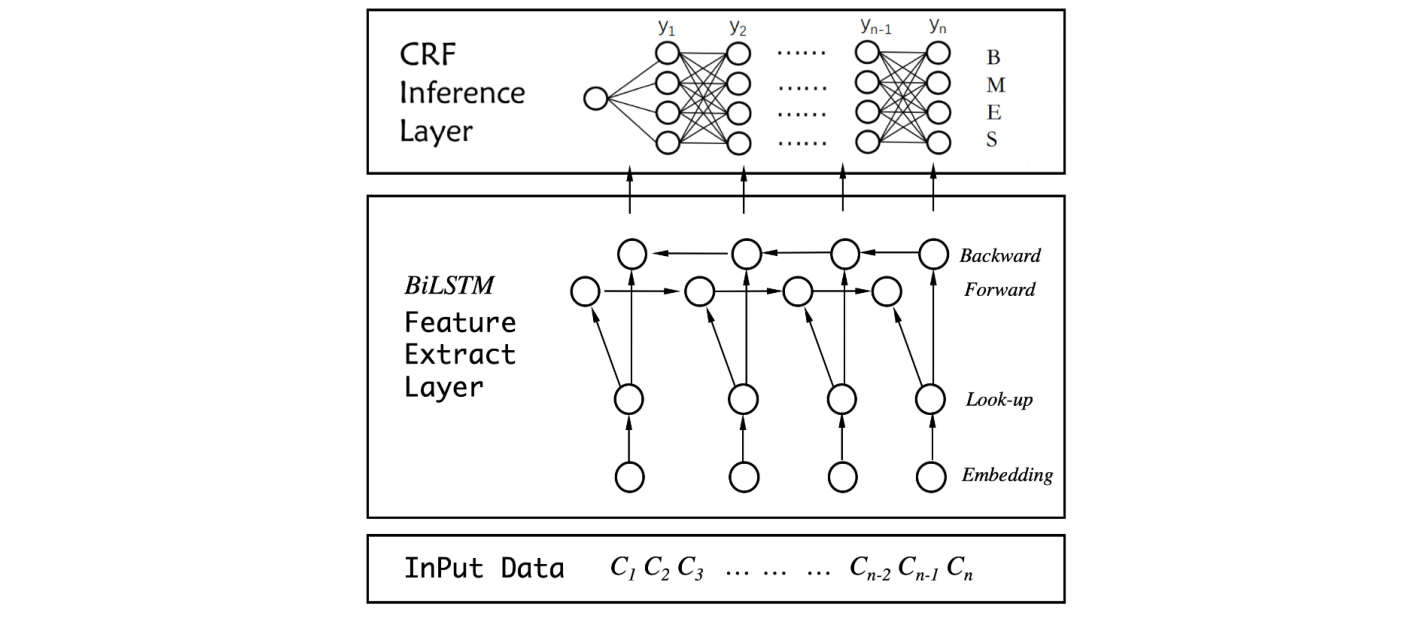
\includegraphics[width=1\textwidth]{figures/model.pdf}
    \end{center}
    \caption{The overview of BiLSTM-CRF model structure}
    \label{fig:overall_model}
\end{figure*}


\subsection{Part-of-speech Tagging}
\label{sec:pos}

目前我们所使用的词性标注,基本上都是以「假设数据集正确」来做的,为了更好的符合数据集的结果,我们将数据集进行分析,并且建立一个简易的知识图谱来做词与词性之间的对应。

我们发现一些棘手的例子,在数据集中,有很多数据会有多种词性标注,故我们倾向于预测数据集中出现最多的那种词性。因为若用模型来预测很容易被误导而训练出很差的效果,所以牺牲一部分「错误的正确性」算是相对合理的。

最原始模型基于所有见过的词进行出现频率上的统计,这在撇除分词效果(直接将 gold 分词结果读入当做模型输入),就可以直接达到95\%左右的准确度。我们倾向于预测所有没出现过的词为名词,毕竟专有名词经过我们统计是最有可能没有出现过的。由于因为输入之分词与评价的集合完全相同,这相当于计算 precision 和 recall 的分母相同,故 precision、recall、f1-score 会呈现完全相同的结果。

之后基于此模型在加上规则,这在数据很脏的时候特别有效,毕竟很多在词性标注的标准中,我们课堂使用的标准特别的「特殊」,所以若尝试使用外部标准,反而会使效果下降,而若使用机器学习,则会「教坏」它。随著规则的增多,提高了几个百分点,毕竟原先的效果已经很好了。



\section{实验内容}
\label{sec:experiment}

最一开始当然是从观察数据开始,并且先将数据处理成可以训练的模式。

我们主要处理三阶段的可训练数据。
第一个就是处理成分词用的训练数据,将数据转换为针对每一个字的四分类问题,在段落~\ref{sec:purpose}也提过,我们所预测的集合为\{B, M, E, S\}。字的部份我们就先不做处理,保留之后转成各种不同的 embedding 表示。
第二阶段数据则是给词性标注的数据,毕竟我们是两个任务并行进行的,但词性标注必须依赖先有分词的结果,故我们将词性标注的 gold 数据处理后形成模拟的分词结果(不直接使用分词的 gold 数据处理,主要是因为分词的数据连<sub> <sup>之类的 tag 都被搞坏了,根本没办法用)。
第三阶段数据是在最终的文本数据提供之前,先利用现有数据还原成原始文章的形式,这是用于测试从无到有的模型输出效果,之后待最后的目标文档提供后只要直接替换这边就可以快速的套用并输出结果。

再来,则是模型的搭建与训练和测试,这部份在前面的段落~\ref{sec:principle}中有详细的叙述。

最后是模型的评价,原先使用了所提供的评价脚本,却发现里面有很多的坑,特别是因为数据中的"//w"和"</sup>"这类数据会被误判成词性,还有空白行也会一同被纳入评测,这导致最后评分出来的表现有很大的误差,故为了保险起见还是针对了这部份进行我们自己版本的改正。

\subsection*{Detail of Word Segmentation}

在分词过程中,测试了CRF单模型,Embed使用了One-Hot, TF-IDF, FastText.

因为在测试过程中发现用预训练词向量效果不好,就没有测试基于Bert或者ELMo的实验。

在跑单CRF过程中,因为输入的是一个句子数*句子长度*特征数的一个三维矩阵。
当利用最大句子长度对齐时,在特征数较多的情况下(即One-Hot)会导致Memory Error。
例如训练集6106句,最大长度1060,One-Hot 2868维度。用 int16 存储,需要 68GB 内存,实际测试中用了int32内存直接打到120GB+。
故在处理这个情况下, 使用了reshape.

另外,在分词这个任务,除了最基本的 MASK 操作之外,实际上带有一个隐藏的条件,即句尾一定分词。
虽然为了学习到上下文信息,不易直接将句尾字符舍去,但在评测过程中,需要手动更改。

因为使用单模型,效果较为一般,为了获得更多上下文信息,在 encoder 层按常规接了一个 BiLSTM。

实验下来,效果比较稳定。像单模型 CRF,训练集和开发集偏差有将近25\%, 而 BiLSTM-CRF 模型偏差在5\%以内。

\section{实验结果}
\label{sec:result}

(描述实验结果并分析原因)

\subsection*{Word Segmentation}

在训练集、开发集与测试集数据中测试结果。(表~\ref{tab:cws_result})

\begin{table}[htbp!]
    \centering
    \begin{tabular}{llccccccccc}
    \toprule
        \multicolumn{1}{c}{\multirow{2}{*}{Model}} & \multirow{2}{*}{Param}      & \multicolumn{3}{c}{Train Set}     & \multicolumn{3}{c}{Dev Set}           & \multicolumn{3}{c}{Test Set}          \\
        \multicolumn{1}{c}{}                       &                             & P             & R        & F1     & P             & R        & F1         & P             & R        & F1         \\
        \midrule
        CRF      & default                                                       & 100.00        & 100.00   & 100.00  & 100.00       & 100.00   & 100.00     & 100.00        & 100.00   & 100.00     \\
    \bottomrule
    \end{tabular}
\caption{Word segmentation (in \%)}
\label{tab:cws_result}
\end{table}

\subsection*{Part-of-speech Tagging}

\subsubsection*{Test on the gold word segmentation result}

在这个测试之中,排除了分词错误的可能性,利用从 testset1 中的 test\_pos1.txt 中提取出分词结果(不使用 test\_cws1.txt 是因为里面的 tag 全是乱的完全无法使用)。(表~\ref{tab:pos_on_gold_cws})

\begin{table}[htbp!]
    \centering
    \begin{tabular}{lccc}
    \toprule
        Method          & F1-Score on Train Set  & F1-Score on Dev Set   & F1-Score on Test Set \\
    \midrule
        Pure Mapping    & 97.98                  & 95.57                 & 95.39                \\
        Add Rules       & -                      & -                     & 95.83                \\
        Even More Rules & 97.98                  & 96.06                 & 95.86                \\
    \bottomrule
    \end{tabular}
\caption{Part-of-speech tagging on Gold CWS (in \%) (precision = recall = f1-score)}
\label{tab:pos_on_gold_cws}
\end{table}

% \subsection*{Overall Test}

% 将所有测试文档还原成原始文档进行分析的结果。(表~\ref{tab:pos_with_cws})

% \begin{table}[htbp!]
    \centering
    \begin{tabular}{llccccccccc}
    \toprule
        \multicolumn{2}{c}{Experiment}    & \multicolumn{3}{c}{Train Set}  & \multicolumn{3}{c}{Dev Set} & \multicolumn{3}{c}{Test Set}  \\
        CWS Method      & POS Method      & P     & R     & F1             & P     & R     & F1          & P     & R     & F1            \\
    \midrule
        CRF             & With Rule       & 95.39 & 95.39 & 95.39          & 95.39 & 95.39 & 95.39       & 95.39 & 95.39 & 95.39         \\
    \bottomrule
    \end{tabular}
\caption{Entire process result from raw article to evaluation (in \%)}
\label{tab:pos_with_cws}
\end{table}


\section{误差分析}
\label{sec:analysis}

(对bad case进行分析)


一开始花了挺多时间在检查F1 score一致性问题上,一致性主要要注意MASK,还有句尾一定分词这个隐藏的条件,另外给的评测脚本和自己写的f1还是有些偏差,但无伤大雅。

到最后开始调模型的时候发现单模型CRF tf-idf效果竟然比One HOT还差。

TF IDF的思路是先做一个窗口获得附近centre word 附近n gram词汇信息,做相应的词频转换。然后丢到sklearn的pipeline中做tf-idf的转换。

因为TF IDF 测试集需要和训练集对齐,在这个处理上把未出现的词都塞到最后一个word的dict中,赋予所有词频为0.

所以一开始怀疑是不是训练集和开发集对齐发生错误,毕竟33\%左右的正确率基本上意味着random。不过因为时间关系,后面就没去check了。

同样替换embed 为常见的预训练词向量,比如说FastText,Glove, ELMo, Bert。

本来想把实验做做完,但做FastText下来效果很差,就直接改BiLSTM-CRF了。

总的来说,在实验过程中TF-IDF训练效果明显低于正常值,且其训练集基本上达到最优效果,很有可能是测试集合训练集特征为对应上。


\section{思考题}
\label{sec:question}

\paragraph{1. NER 部分存在同一个词被多个 NER 嵌套的情况,但是序列标注的 NER 模型对于一个词往往只能有一个 NER 标注,如何解决该问题?}

e.g:[[肺动脉]bod 狭窄]sym

\paragraph{2. 分词任务与 pos/ner 任务其实是紧密相关的,如果在分词阶段出现错误,该部分误 差就会传递下去,如何解决该问题?}

\paragraph{3. 训练数据量十分有限,在不使用人工标注的情况下,如何扩充数据量,并进一步优 化模型效果?}


\section{实验分工及感想}
\label{sec:conclusion}

一开始也没有太特别的分工,主要先阅读一些相关的论文以及逐行研究目前流行之分词工具的底层源代码来收集灵感,接著一起决定要使用什么样的模型、使用哪些 library,并且拟定大方向架构。后来因为我们这学期修了太多扎实的课,包含数门信科的自然语言处理课程,导致时间被压缩的很紧迫,故决定并行动工,由姜慧强实现分词、李大为来做预处理与实现词性标注。相关工作细节皆公开透明开源于 \fnurl{Github}{https://github.com/pku-nlp-forfun/CWS_POS_NER} 上。

由于所提供的数据与评测脚本实在太过于草率,故在实作时姜慧强也花了很多时间校正了评测脚本,让在训练模型时不致于被错误的指标误导而往错误的方向优化。由于数据基本上已经脏到不能当做一般数据来使用,也不可能找其他数据集来训练,因为所基于的标准完全不同,也没有很多特有的东西,比如"\$\$\_"之类的东西。所以一旦想要追求模型表现,那就不可能做出能通用于其他语料的版本。那我们最后决定主要倾向针对本次任务进行优化,并且不使用任何外部数据。但由于数据量对于模型训练还是偏少,故过度的追求模型表现只是纯粹的自我打击,也让我们学会了,如果是任务结果导向,能跳脱机器学习的迷思也许才是其中的关键,仔细去看结巴分词的实现,里面也有很多正则表达式,毕竟并不是所有任务、数据都适合机器学习。


\bibliographystyle{acm}
\bibliography{citedbibtex}

\end{document}